
\documentclass[10pt]{article}% insert '[draft]' option to show overfull boxes
\usepackage{amsmath}
\usepackage{amssymb}
\usepackage{float}
\usepackage{graphicx}
%\usepackage[margin=1cm]{caption}
\usepackage{subfig}
\usepackage{setspace}
\usepackage[margin=1.0in]{geometry}
\usepackage{breqn}

\usepackage{etoolbox}
\providetoggle{HOT}
\settoggle{HOT}{false}

\usepackage{color}
\definecolor{gray1}{gray}{0.6}
\definecolor{gray2}{gray}{0.3}


 % Define commands to assure consistent treatment throughout document
% \newcommand{\eqnref}[1]{(\ref{#1})}
% \newcommand{\class}[1]{\texttt{#1}}
% \newcommand{\package}[1]{\texttt{#1}}
% \newcommand{\file}[1]{\texttt{#1}}
% \newcommand{\BibTeX}{\textsc{Bib}\TeX}

\title{Backward Euler Time Integration Truncation Error}

\author{Tyrone Phillips, Ph.D.}
\begin{document}

\maketitle

\section*{Truncation error analysis }



%\begin{center}
\begin{picture}(600, 60)
\put(20,20) {\line(0,1){30}}
\put(100,20) {\line(0,1){30}}
\put(180,20) {\line(0,1){30}}
\put(260,20) {\line(0,1){30}}
\put(340,20) {\line(0,1){30}}

\put(20,10) {\vector(1,0){380} }
\put(410,10) {\makebox(0,0){$t$} }

%\put(140,6) {\line(0,1){8}}

\put(20,8) {\line(0,1){4}} 
\put(20,2) {\makebox(0,0){$$}}
\put(100,8) {\line(0,1){4}} 
\put(100,2) {\makebox(0,0){$$}}
\put(180,8) {\line(0,1){4}}
\put(180,2) {\makebox(0,0){$n-3/2$}}
\put(260,8) {\line(0,1){4}}
\put(260,2) {\makebox(0,0){$n-1/2$}}
\put(340,8) {\line(0,1){4}}
\put(340,2) {\makebox(0,0){$n+1/2 $}}

\put(60,35) {\makebox(0,0){$\circ$}}
\put(60,45) {\makebox(0,0){n-3}}

\put(140,35) {\makebox(0,0){$\circ$}}
\put(140,45) {\makebox(0,0){n-2}}

\put(220,35) {\makebox(0,0){$\circ$}}
\put(220,45) {\makebox(0,0){n-1}}

\put(300,35) {\makebox(0,0){$\circ$}}
\put(300,45) {\makebox(0,0){n}}



\end{picture}
%\end{center}


\[ \frac{\partial \phi}{\partial t} = \frac{\phi^{n+1/2} - \phi^{n-1/2}}{\Delta t} \]
where
\[ \phi^{n+1/2} = \phi^{n} + \frac{\Delta t_n}{\Delta t_n + \Delta t_{n-1}}\left( \phi^n - \phi^{n-1}\right), \]
\[ \phi^{n-1/2} = \phi^{n-1} + \frac{\Delta t_{n-1}}{\Delta t_{n-1} + \Delta t_{n-2}} \left( \phi^{n-1} - \phi^{n-2}\right),\]
and
\[ \Delta t_n = t_{n+1/2} - t_{n-1/2}.\]
Simplified is
\begin{equation}
\left(\frac{\partial \phi}{\partial t}\right)^n = \left(\phi^n - \phi^{n-1}\right)\left( \frac{1}{\Delta t_n} + \frac{1}{\Delta t_n + \Delta t_{n-1}}\right) - \left( \phi^{n-1} - \phi^{n-2}\right) \frac{\Delta t_{n-1}}{\Delta t_n(\Delta t_{n-1} + \Delta t_{n-2}) }.
\end{equation}

Taylor series expansions about $n$
\[
\phi^{n-1} = \phi^n 
  - \left( \frac{\Delta t_n}{2} + \frac{\Delta t_{n-1}}{2}\right) \frac{\partial \phi}{\partial t}
  + \frac{1}{2}\left( \frac{\Delta t_n}{2} + \frac{\Delta t_{n-1}}{2}\right)^2 \frac{\partial^2 \phi}{\partial t^2}
  - \frac{1}{6}\left( \frac{\Delta t_n}{2} + \frac{\Delta t_{n-1}}{2}\right)^3 \frac{\partial^3 \phi}{\partial t^3}
  + O(\Delta t^4)
\]

\[
\phi^{n-1} = \phi^n 
  - \left( \frac{\Delta t_n}{2} + \Delta t_{n-1} + \frac{\Delta t_{n-2}}{2}\right) \frac{\partial \phi}{\partial t}
  + \frac{1}{2}\left( \frac{\Delta t_n}{2} + \Delta t_{n-1} + \frac{\Delta t_{n-2}}{2}\right)^2 \frac{\partial^2 \phi}{\partial t^2}
\]
\[
  - \frac{1}{6}\left( \frac{\Delta t_n}{2} + \Delta t_{n-1} + \frac{\Delta t_{n-2}}{2}\right)^3 \frac{\partial^3 \phi}{\partial t^3}
  + O(\Delta t^4)
\]
substituted into the backward Euler calculation results in the truncation error
\[
  \tau_h(\phi) = -\frac{\partial^2 \phi}{\partial t^2}\left(\frac{ 12\Delta t_n^2 + 6\Delta t_n \Delta t_{n-1} - 12 \Delta t_{n-2}^2 - 6 \Delta t_{n-1} \Delta t_{n-2} }{48 \Delta t_n}\right)
\]
\[
  -\frac{\partial^3 \phi}{\partial t^3}\left( \frac{ -2\Delta t_n^3 - 2\Delta t_n^2\Delta t_{n-1} + 5 \Delta t_n \Delta t_{n-1}^2 + 3\Delta t \Delta t_{n-1} \Delta t_{n-2} + 6 \Delta t_{n-1}^3 + 5 \Delta t_{n-1}^2\Delta t_{n-2} + \Delta t_{n-1}\Delta t_{n-2}^2  }{48 \Delta t_n} \right) + O(\Delta t^3)
\]
and if $\Delta t = \Delta t_{n} = \Delta t_{n-1} = \Delta t_{n-2}$
\begin{equation}
\tau_{eq,h}(\phi) = -\frac{\partial^3 \phi}{\partial t^3} \frac{\Delta t^2}{3} + O(\Delta t^3).
\end{equation}

The analytic truncation error derivations are confirmed by comparison to the exact truncation error using a solution to Burgers' equation in the following figures.


\begin{figure}[H]
  \begin{minipage}{0.5\textwidth}
    \centering
    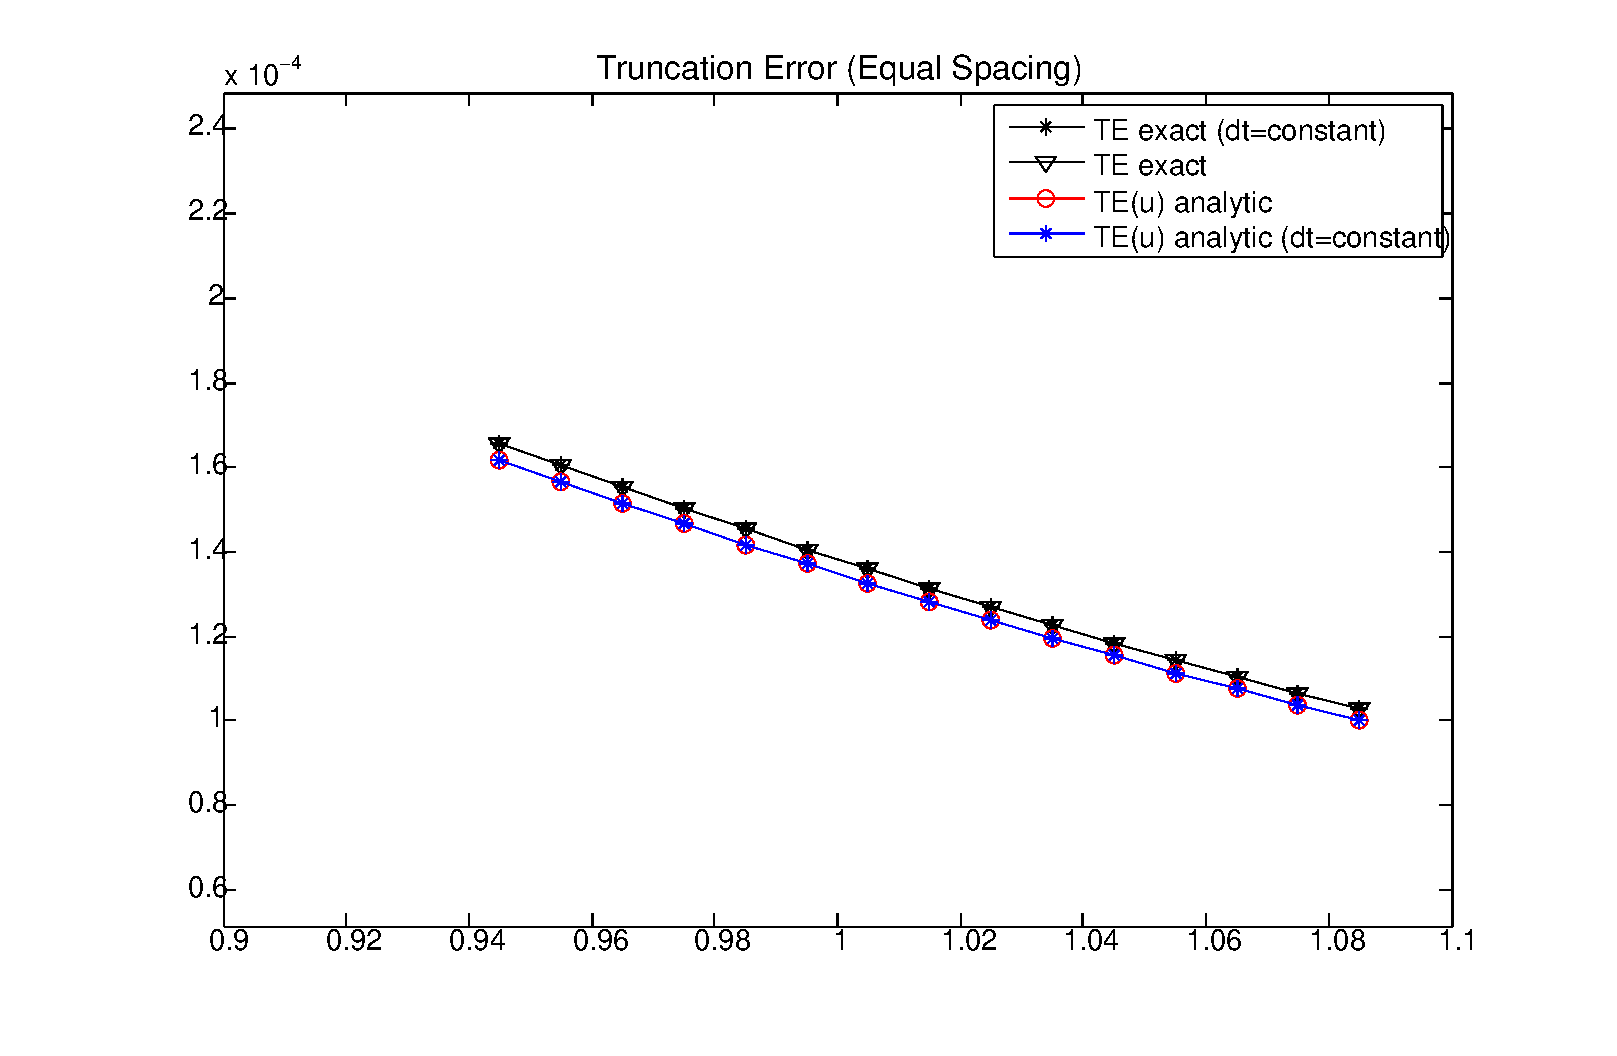
\includegraphics[width=3.5in]{TE_ex_vs_anytc_equalspacing}
  \end{minipage}
  \hfill
  \begin{minipage}{0.5\textwidth}
    \centering
    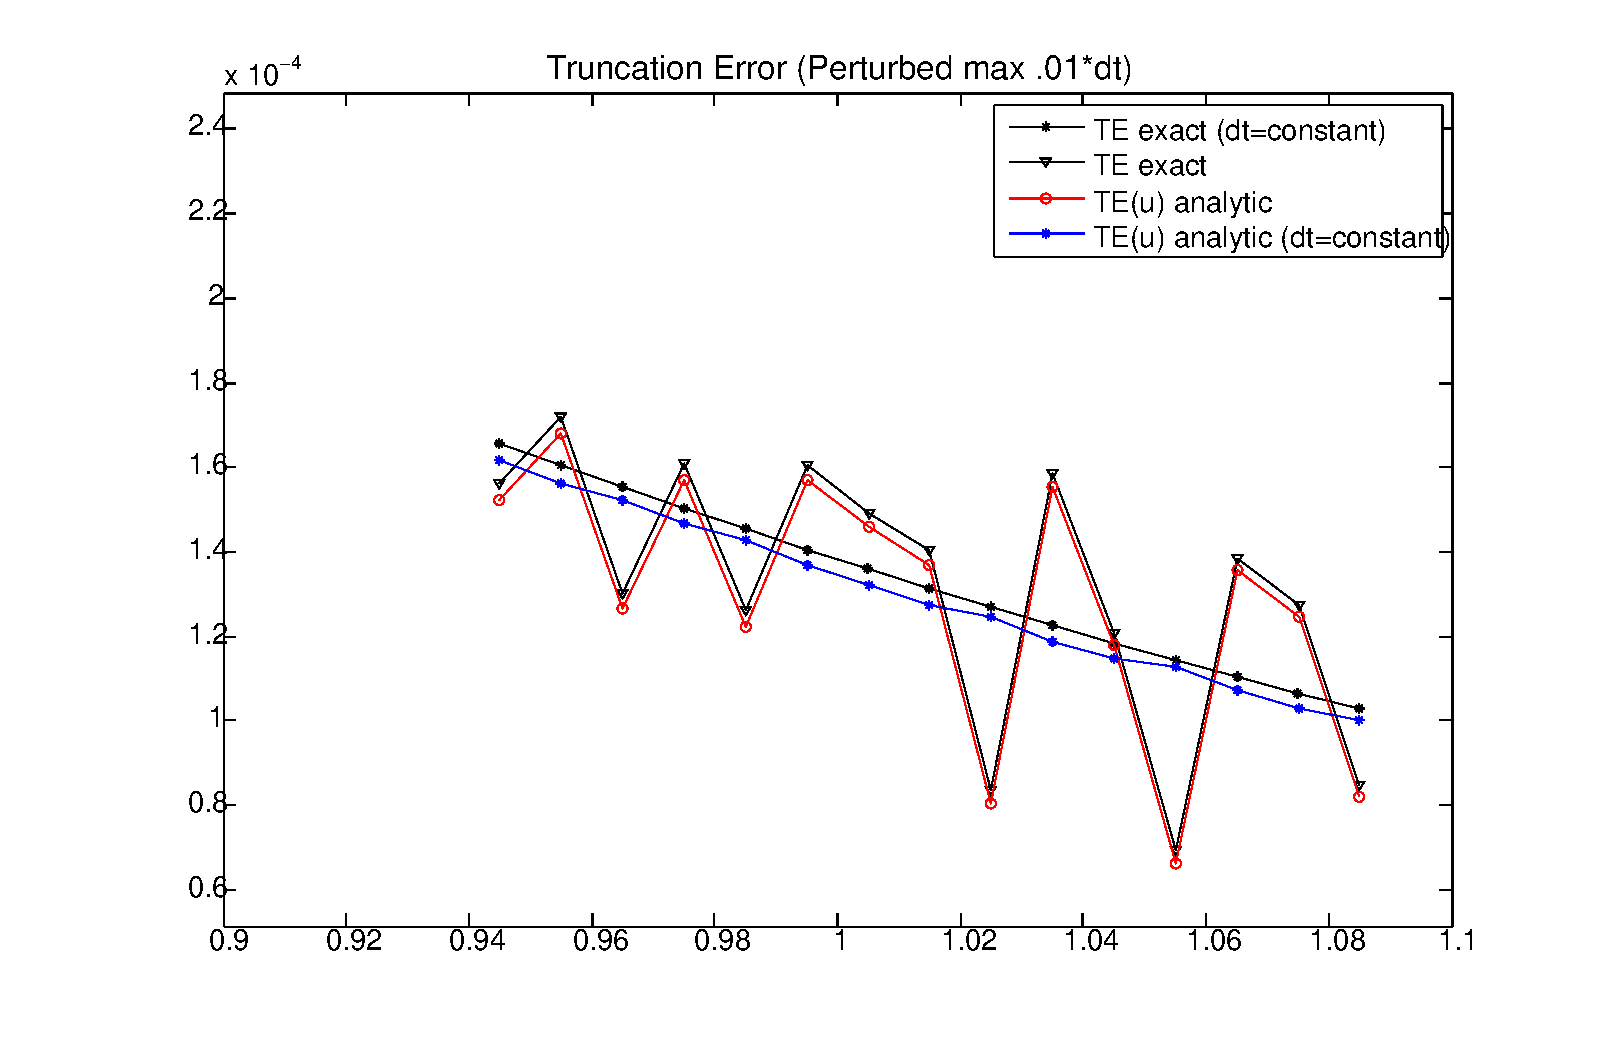
\includegraphics[width=3.5in]{TE_ex_vs_anytc_01}
  \end{minipage}
\end{figure}
\begin{figure}[H]
    \centering
    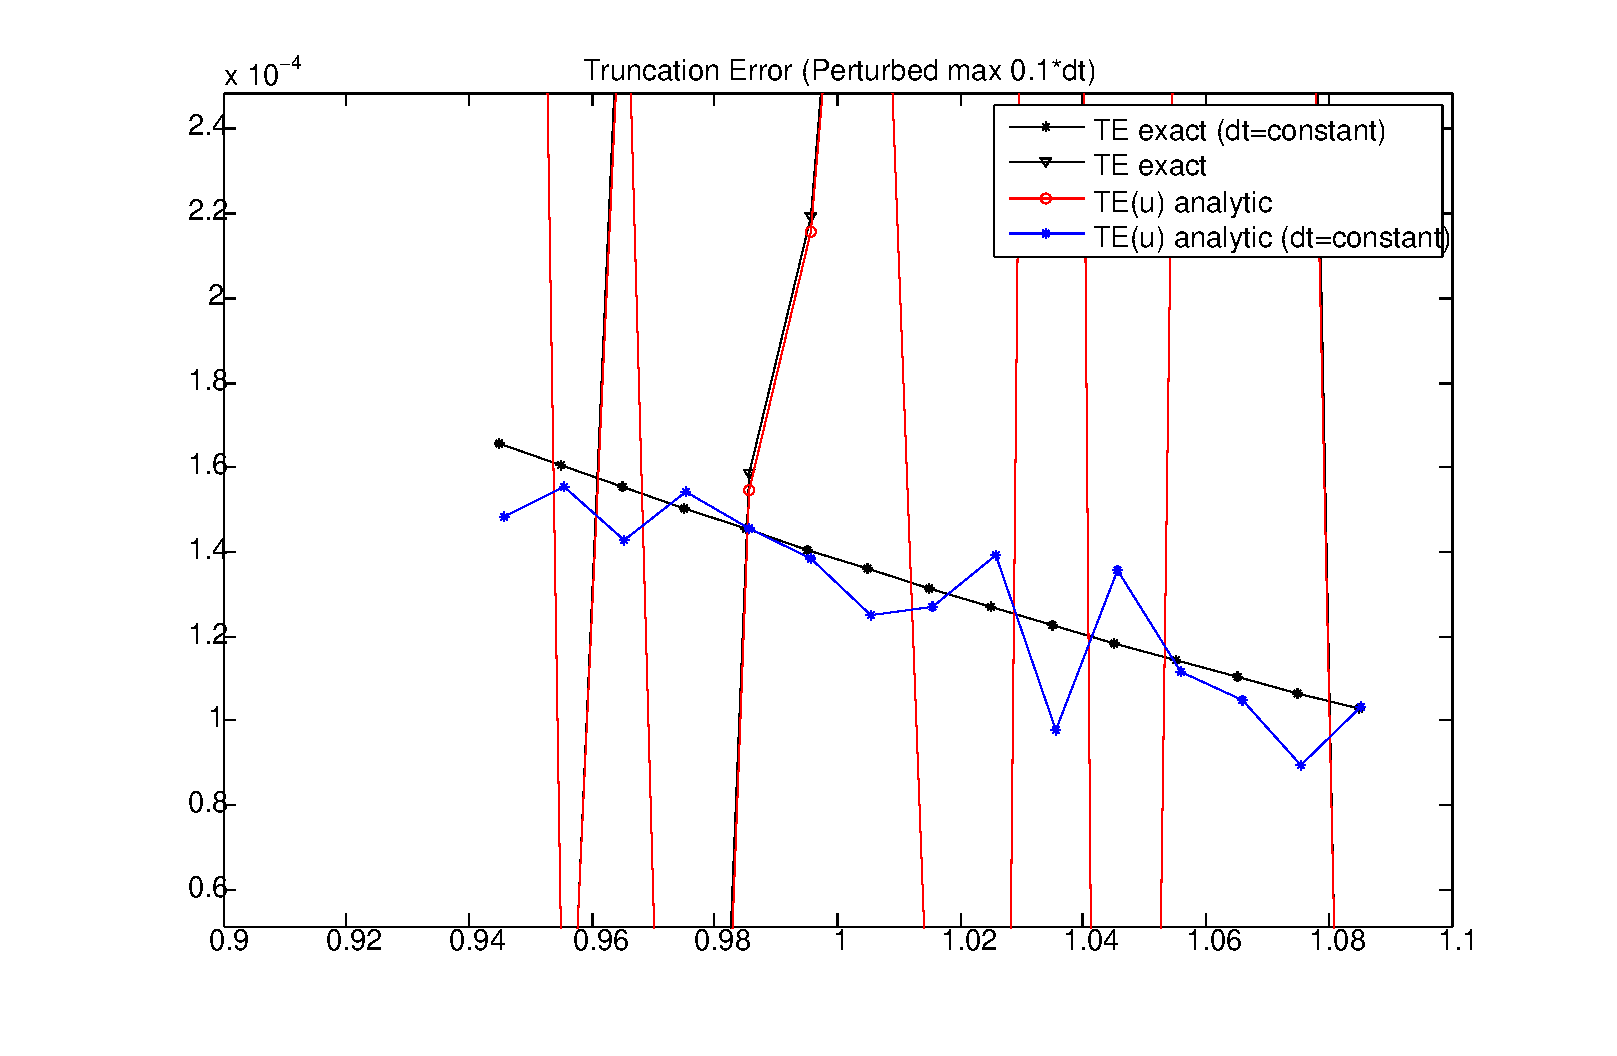
\includegraphics[width=3.5in]{TE_ex_vs_anytc_1}
    \caption{Verification of analytic truncation error derivations}
\end{figure}





\break

\section*{Truncation Error Estimation}
To estimate the truncation error a higher order reconstruction is required which takes into account the non-equal spacing:
\[ p(\Delta t) = c_0 + \Delta t c_1 + \Delta t^2 c_2 + \Delta t^3 c_3 \]
with the constraints 
\[p(0)=\phi_n,\]
\[p\left(\frac{\Delta t_n}{2} + \frac{\Delta t_{n-1}}{2}\right)=\phi_{n-1},\]
\[p\left(\frac{\Delta t_n}{2} + \Delta t_{n-1} + \frac{\Delta t_{n-2}}{2}\right)=\phi_{n-2},\]
\[p\left(\frac{\Delta t_n}{2} + \Delta t_{n-1} + \Delta t_{n-2} + \frac{\Delta t_{n-3}}{2}\right)=\phi_{n-3}.\]

Truncation error estimation methods:
\begin{itemize}
  \item M1a - Analytic truncation error estimation: $\tau_h(\phi) \approx \tau_h(p(\Delta t))$ 
  \item M1b - Direct error calculation: $\tau_h(\phi) \approx \left(\frac{\partial \phi}{\partial t}\right)^n - \frac{\partial p}{\partial t} = \left(\frac{\partial \phi}{\partial t}\right)^n - c_1$
  \item M2a  - Analytic equally-spaced truncation error: $\tau_{eq,h}(\phi) \approx -\frac{\partial^3 p}{\partial t^3} \frac{\Delta t_n^2}{3} = -2 c_3 \Delta t^2$
  \item M2b  - Analytic equally-spaced truncation error: $\tau_{eq,h}(\phi) \approx -\frac{\partial^3 p}{\partial t^3} \frac{\Delta \bar t^2}{3} = -2 c_3 \Delta \bar t^2$
  \item M3a - Smooth grid truncation error: $\tau_{eq,h}(\phi) \approx \frac{3c_0 - 4p(\Delta t_n) + p(2\Delta t_n)}{2\Delta t_n}$
  \item M3b - Smooth grid truncation error: $\tau_{eq,h}(\phi) \approx \frac{3c_0 - 4p(\Delta \bar t) + p(2\Delta \bar t)}{2\Delta \bar t}$

\end{itemize}
For methods M2b and M3b $\Delta \bar t = \frac{1}{N+1}\sum_{i=0}^N \Delta t_{n-i}$.

The estimates are compared to the exact TE in the following figures. From here it is clear that M1a=M1b and M2=M3. The differences between M3a and M3b is due to the averaged $\Delta t$ used to compute the truncation error. Comparing the differences in estimates for method M2b with variable N, $N>=2$ seems to give moderately smooth results. Perhaps $N=3$ is the best choice as it includes the stencil for the higher order reconstruction.

\break
\begin{figure}[H]
  \begin{minipage}{0.5\textwidth}
    \centering
    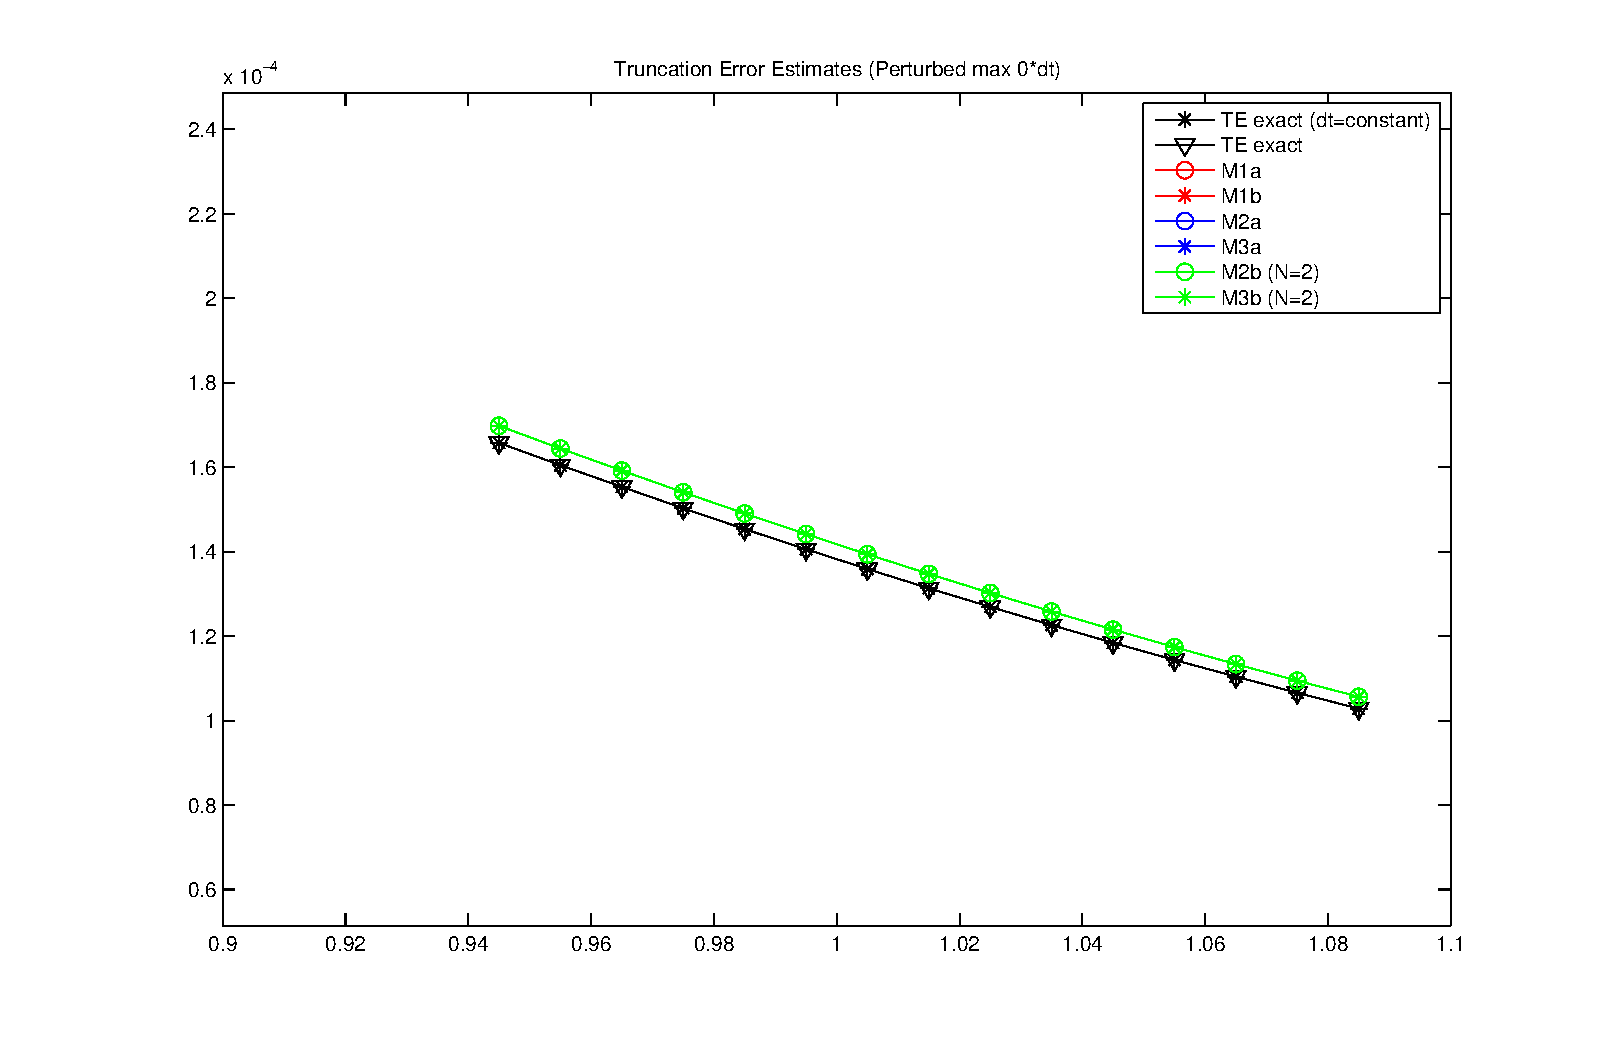
\includegraphics[width=3.5in]{TE_ex_vs_est_equalspacing}
  \end{minipage}
  \hfill
  \begin{minipage}{0.5\textwidth}
    \centering
    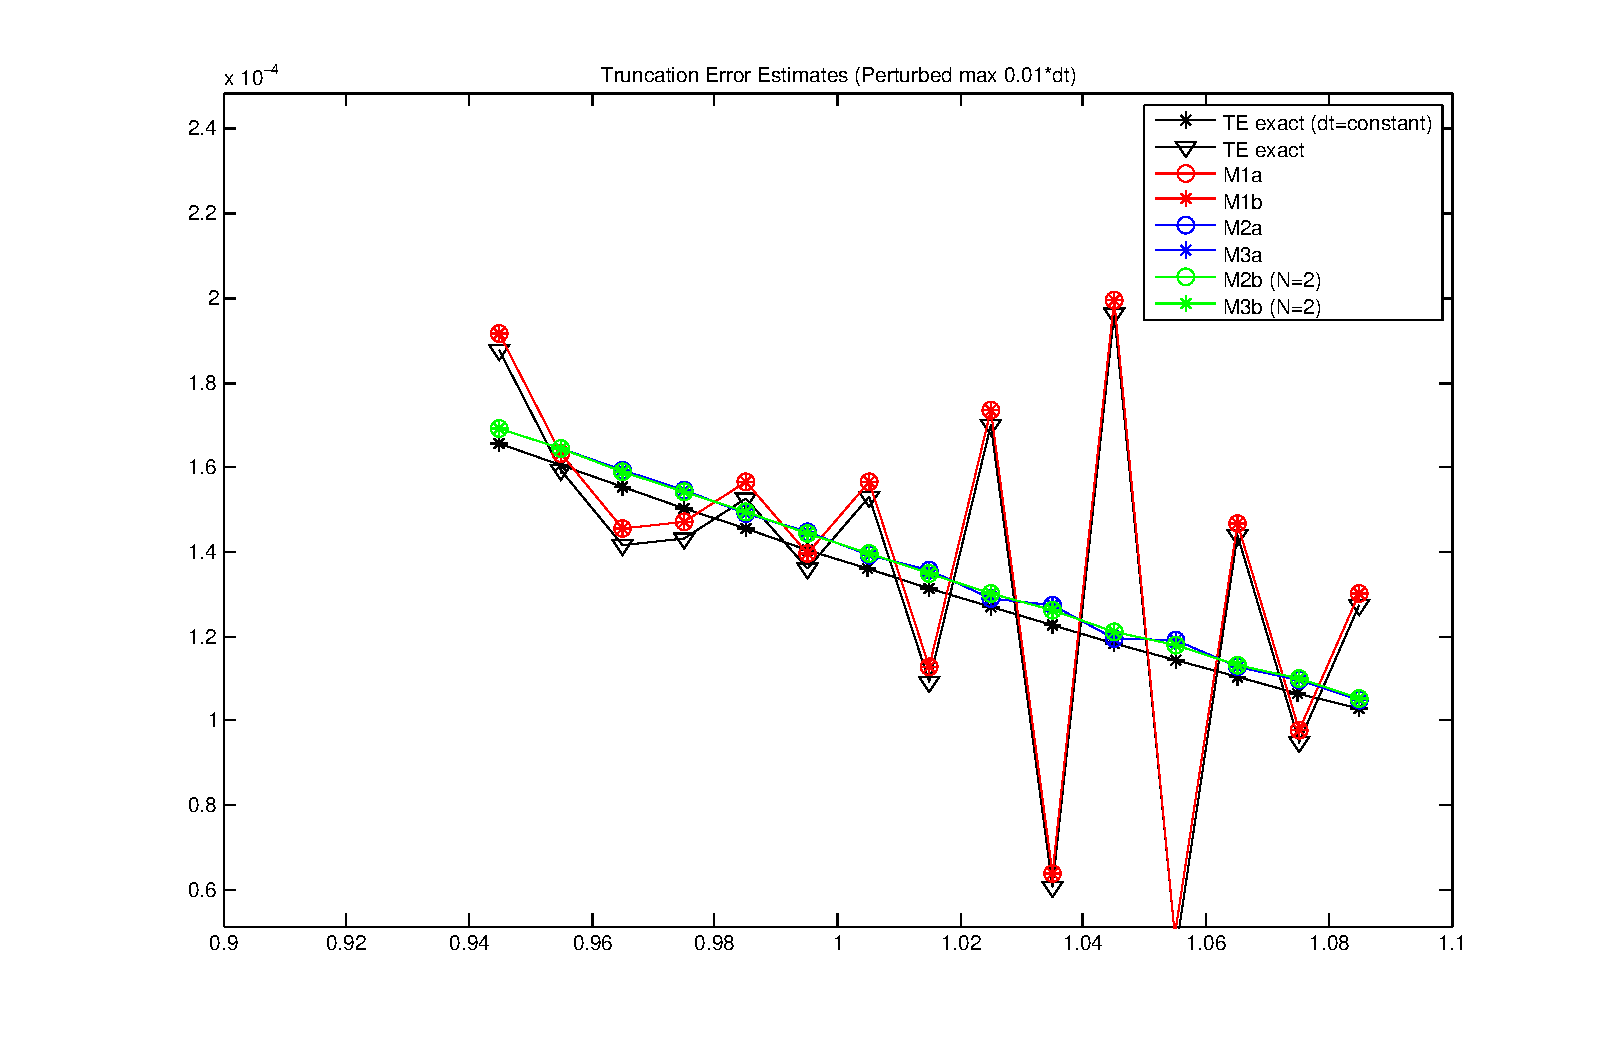
\includegraphics[width=3.5in]{TE_ex_vs_est_01}
  \end{minipage}
\end{figure}
\begin{figure}[H]
  \begin{minipage}{0.5\textwidth}
    \centering
    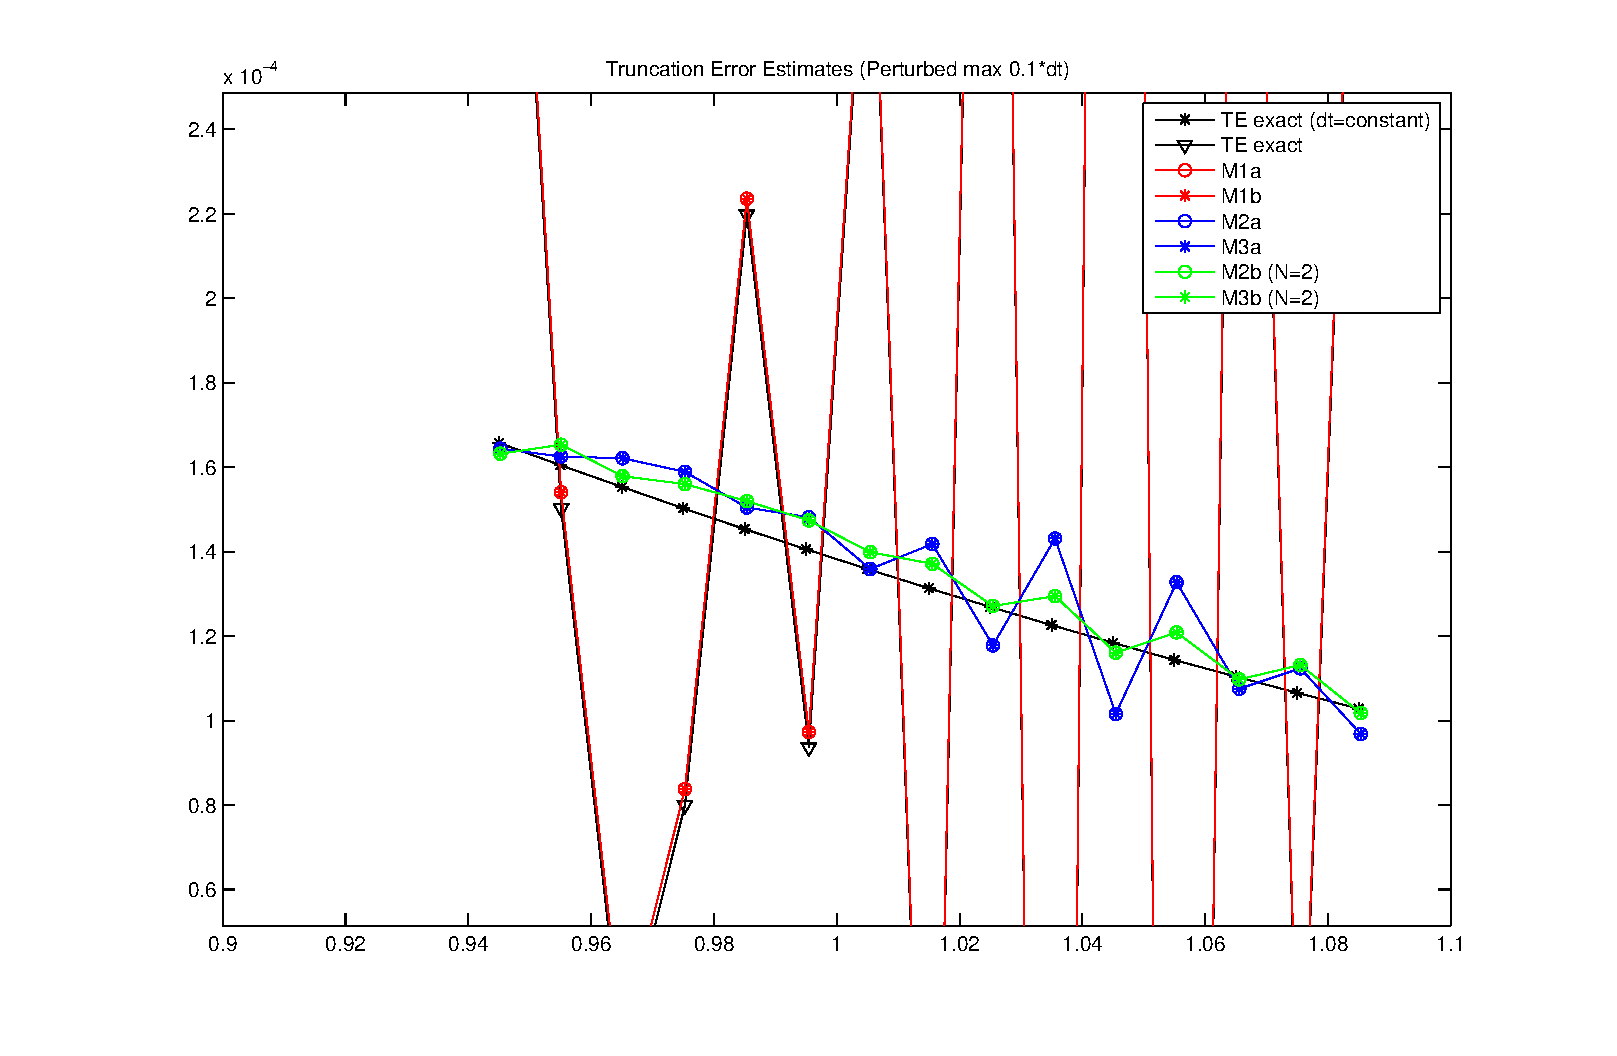
\includegraphics[width=3.5in]{TE_ex_vs_est_1}
  \end{minipage}
  \hfill
  \begin{minipage}{0.5\textwidth}
    \centering
    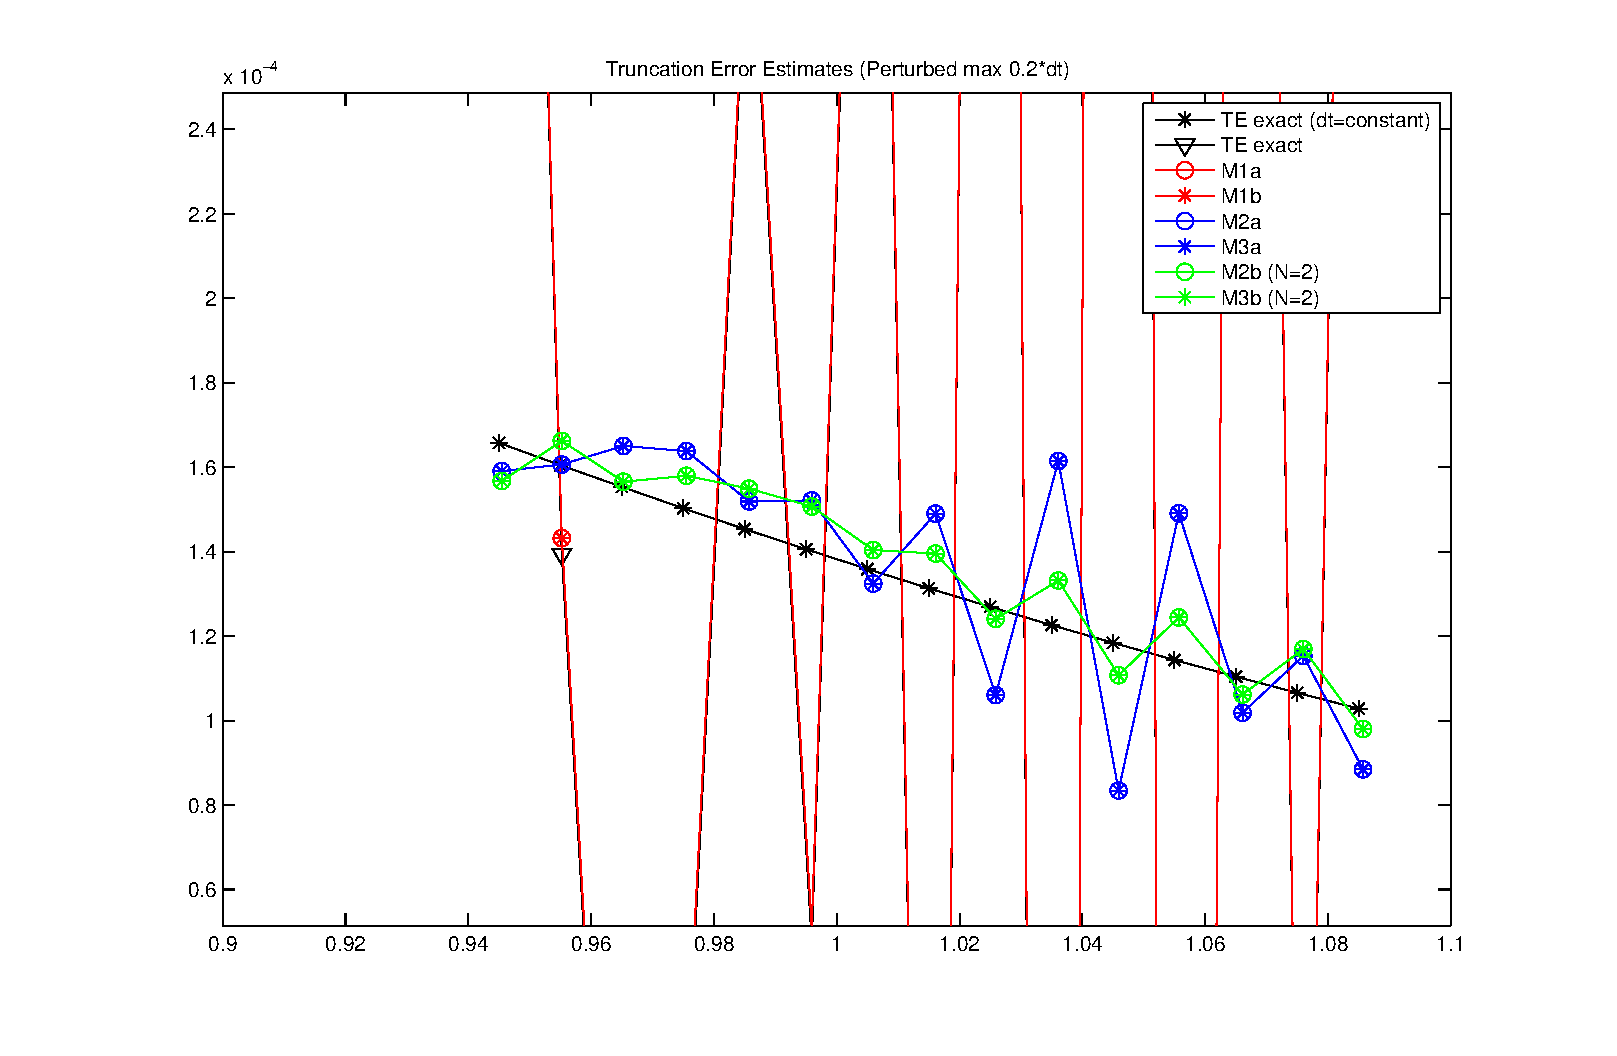
\includegraphics[width=3.5in]{TE_ex_vs_est_2}
  \end{minipage}
\end{figure}

\begin{figure}[H]
    \centering
    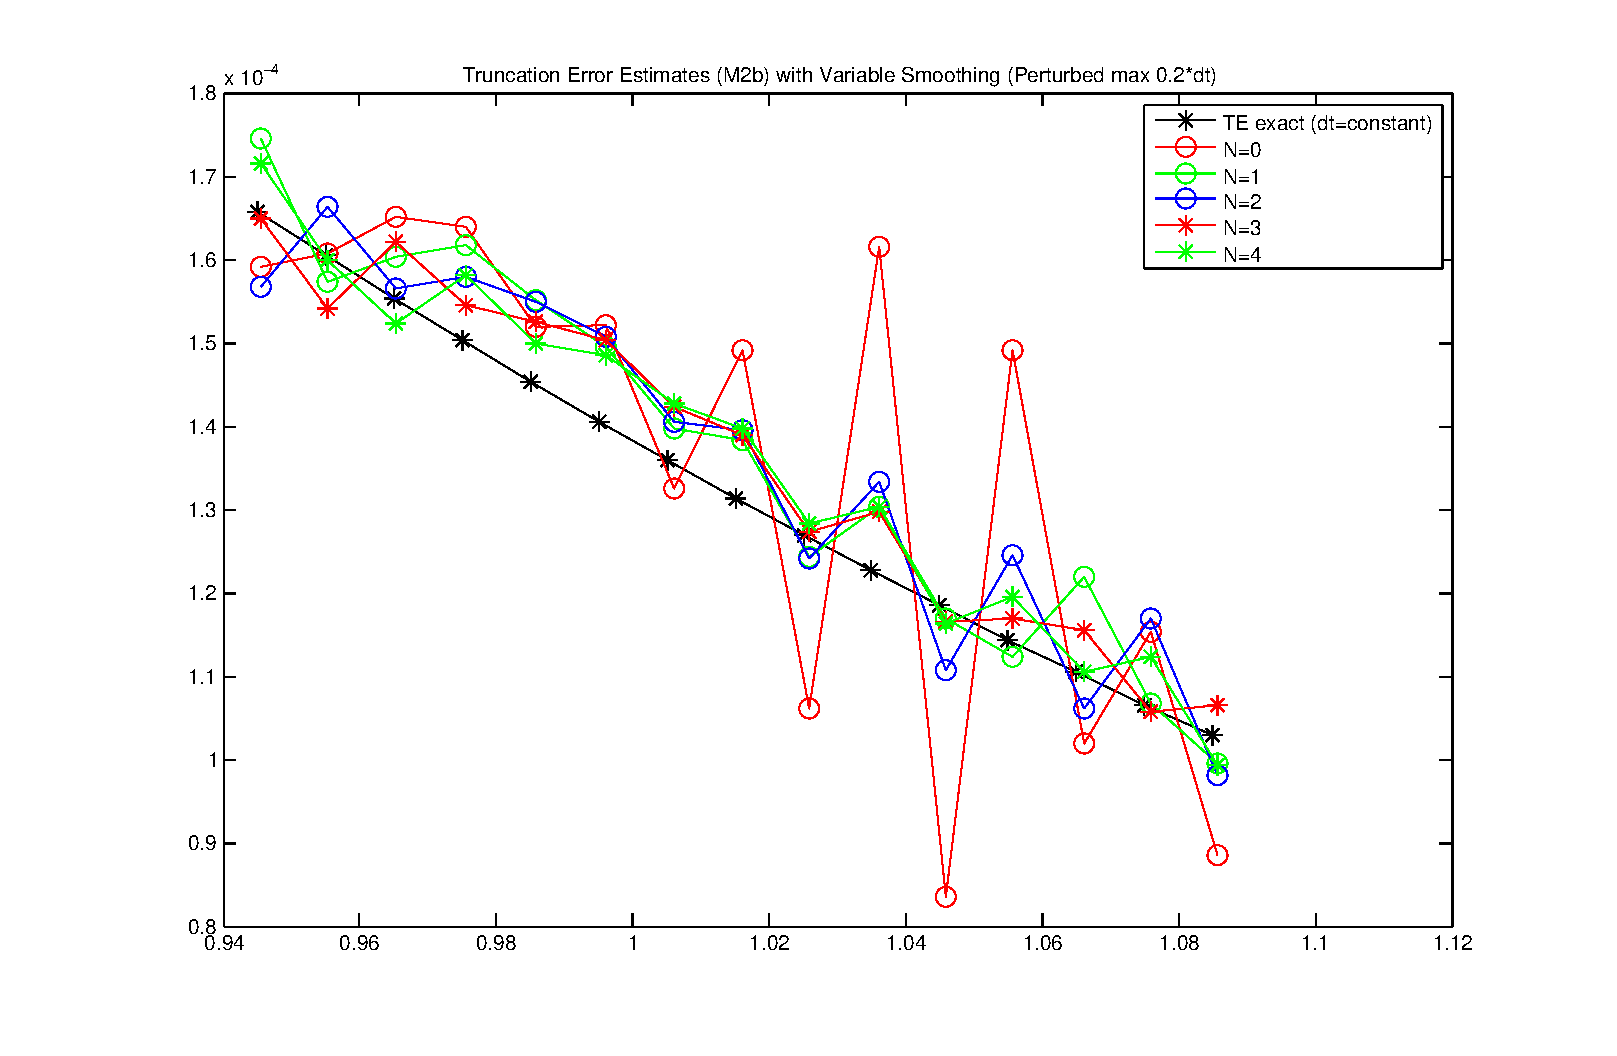
\includegraphics[width=4.5in]{TE_ex_vs_est_varsmoothing}
    \caption{Truncation error estimation comparison}
\end{figure}


\break
\section*{Time Derivative with Better Behaved Truncation Error}
A backward derivative calculation derived using a polynomial fit that includes variable spacing reduces the noise in the exact truncation error. Using the polynomial
\[ p(\Delta t) = c_0 + \Delta t c_1 + \Delta t^2 c_2\]
and solving for the coefficients results in
\[
\left( \frac{\partial \phi}{\partial t} \right)^n = -(\phi^n-\phi^{n-2})\frac{2(\Delta t_n + \Delta t_{n-1}) }{ (\Delta t_{n-1}+\Delta t_{n-2})(\Delta t_n + 2\Delta t_{n-1} + \Delta t_{n-2})  } + (\phi^n-\phi^{n-1}) \frac{ 2(\Delta t_n + 2\Delta t_{n-1} + \Delta t_{n-2}) }{ (\Delta t_n + \Delta t_{n-1})(\Delta t_{n-1} + \Delta t_{n-2}) }
\]

The analytic truncation error is
\[
\tau_h(\phi) = -\frac{1}{24}\frac{\partial^3 \phi}{\partial t^3} (\Delta t_n + \Delta t_{n-1})(\Delta t_n + 2\Delta t_{n-1} + \Delta t_{n-2}  )  + O(\Delta t^3)
\]

The figures below compare the exact truncation error, the analytic truncation error evaluated using the higher order reconstruction and the equal spacing truncation error estimation method M2b with N=3. For equal spacing, the truncation error is identical; however, for the perturbed mesh, the new derivative calculation has truncation error very nearly the same as the equal spacing trucation error. Using this instead of the previous method might result in better adaptive results. Either estimation method M1a and M2b seems a feasible option for driving the time adaption.  

\begin{figure}[H]
  \begin{minipage}{0.5\textwidth}
    \centering
    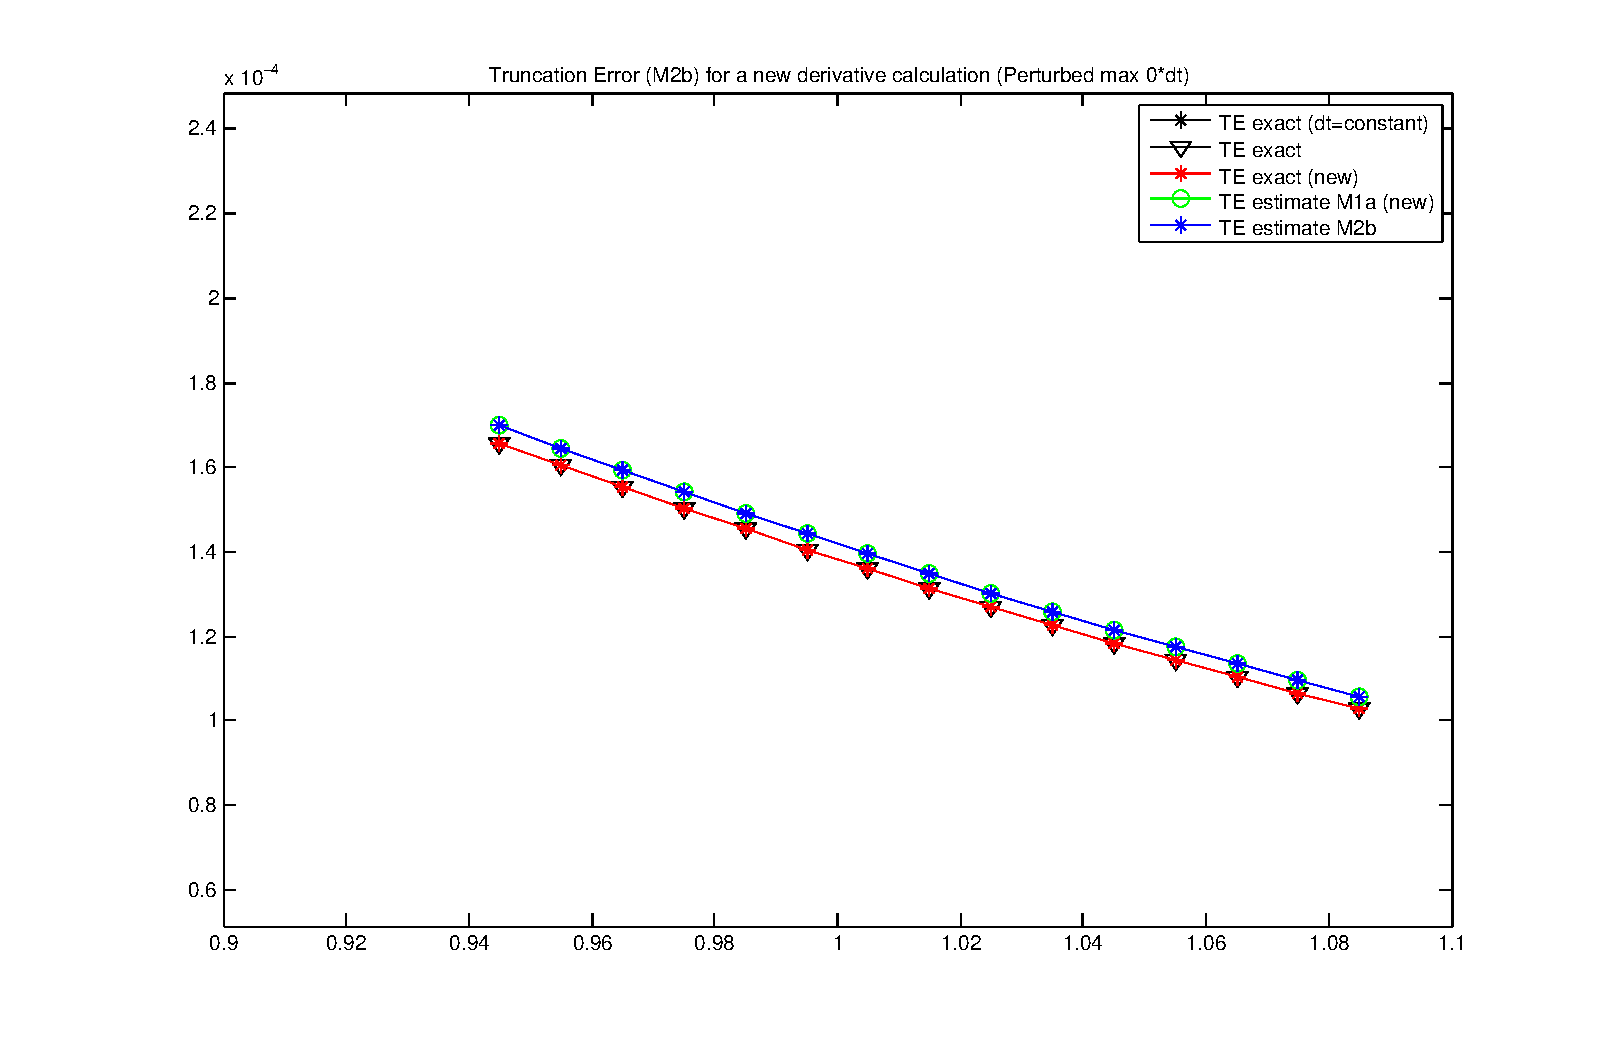
\includegraphics[width=3.5in]{TE_ex_new_extrap_equalspacing}
  \end{minipage}
  \hfill
  \begin{minipage}{0.5\textwidth}
    \centering
    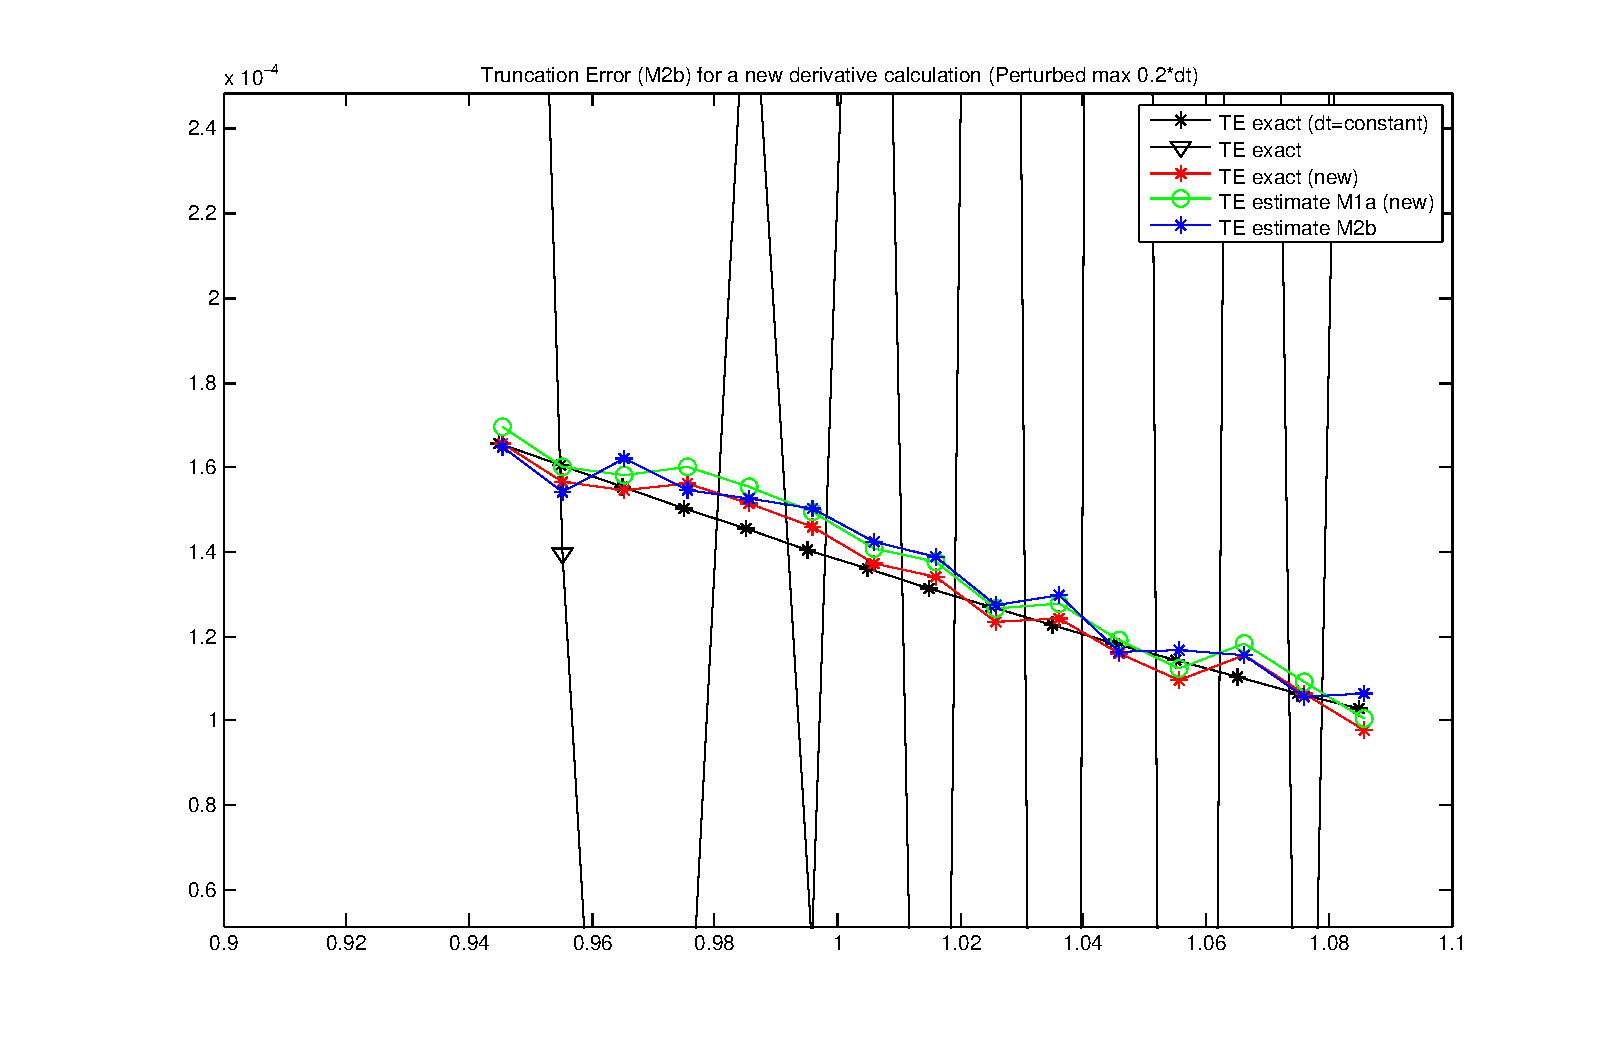
\includegraphics[width=3.5in]{TE_ex_new_extrap_2}
  \end{minipage}
\end{figure}


\end{document}
% - Release $Name:  $ -
